
%  Adaptive Multigrid FSP for the RDME — Talk Slides
%  Aditya Dendukuri

\documentclass[10pt,aspectratio=169]{beamer}

\usetheme{Boadilla}
\usecolortheme{seahorse}
\setbeamertemplate{navigation symbols}{}
\setbeamerfont{frametitle}{size=\normalsize,series=\bfseries}
\setbeamerfont{title}{size=\large,series=\bfseries}
\setbeamertemplate{bibliography item}[text]

\usepackage{pgfpages}
\pgfpagesuselayout{resize to}[physical paper width=33.87cm,physical paper height=19.05cm]

\usepackage{amsmath,amssymb,bm,mathtools}
\usepackage{tikz}
\usetikzlibrary{arrows.meta,positioning,patterns,decorations.pathreplacing}
\usepackage{graphicx}
\usepackage{booktabs}
\usepackage{xcolor}
\usepackage[numbers,sort&compress]{natbib}
\usepackage{pifont}

\graphicspath{{figures/}}

\newcommand{\bx}{\mathbf{x}}
\newcommand{\Znn}{\mathbb{Z}_{\geq 0}}
\newcommand{\E}{\mathbb{E}}
\newcommand{\TV}{\operatorname{TV}}
\newcommand{\Bin}{\operatorname{Bin}}
\newcommand{\calR}{\mathcal{R}}
\newcommand{\calP}{\mathcal{P}}
\newcommand{\norm}[1]{\left\|#1\right\|}
\newcommand{\citeref}[1]{{\scriptsize\textcolor{gray}{#1}}}

\definecolor{fastblue}{RGB}{31,119,180}
\definecolor{slowred}{RGB}{214,39,40}
\definecolor{coarsegreen}{RGB}{44,160,44}
\definecolor{finecolor}{RGB}{214,39,40}
\definecolor{coarsecolor}{RGB}{31,119,180}
\definecolor{intercolor}{RGB}{255,140,0}


\title[Adaptive Multigrid FSP]{%
  Adaptive Multigrid Finite State Projection\\
  for the Reaction-Diffusion Master Equation}
\author{Aditya Dendukuri}
\institute[UCSB]{University of California, Santa Barbara}
\date{}


\begin{document}

\begin{frame}
  \titlepage
\end{frame}


% ================================================================
\section{Setting}
% ================================================================

\begin{frame}[shrink=6]{A probability ODE for stochastic chemical kinetics}

  \begin{columns}[T]
    \begin{column}{0.56\textwidth}
      \textbf{Setting:} $N$ species reacting in a well-mixed vessel.
      State $\mathbf{n}\in\mathbb{Z}_{\geq 0}^N$: molecule counts.
      Reaction $r$ fires at rate $\alpha_r(\mathbf{n})$, shifts state by $\nu_r$.

      \medskip
      \textbf{Joint} probability $p(\mathbf{n},t) = \Pr[N(t){=}\mathbf{n}]$ —
      all species counts simultaneously — satisfies the
      \textbf{Chemical Master Equation (CME)}:
      \[
        \frac{dp}{dt} = A\,p,\qquad A_{\mathbf{n}+\nu_r,\mathbf{n}} = \alpha_r(\mathbf{n}).
      \]

      \begin{block}{Finite State Projection \citeref{[Munsky \& Khammash 2006]}}
        Truncate to $\mathcal{S}\subset\mathbb{Z}_{\geq 0}^N$;
        solve $\dot{p}_\mathcal{S} = A_\mathcal{S}\,p_\mathcal{S}$.\\
        Error $=$ probability flux leaving $\mathcal{S}$ — bounded at runtime.\\
        Expand $\mathcal{S}$ only when flux exceeds tolerance.
      \end{block}

      \textbf{Challenge:} $|\mathcal{S}|$ grows combinatorially.
      Coupling $K$ voxels makes this $n_{\max}^K$ — dramatically worse.
    \end{column}
    \begin{column}{0.40\textwidth}
      \begin{center}
      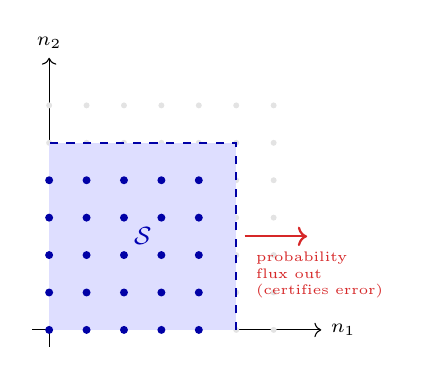
\begin{tikzpicture}[scale=0.72]
        \draw[->] (-0.3,0) -- (4.8,0) node[right,font=\scriptsize]{$n_1$};
        \draw[->] (0,-0.3) -- (0,4.8) node[above,font=\scriptsize]{$n_2$};
        \foreach \i in {0,...,6}
          \foreach \j in {0,...,6}
            \fill[gray!22] (0.66*\i,0.66*\j) circle (1.5pt);
        \fill[blue!13] (0,0) rectangle (3.3,3.3);
        \draw[blue!65!black,thick,dashed] (3.3,0) -- (3.3,3.3) -- (0,3.3);
        \foreach \i in {0,...,4}
          \foreach \j in {0,...,4}
            \fill[blue!65!black] (0.66*\i,0.66*\j) circle (2pt);
        \node[blue!70!black,font=\small] at (1.65,1.65) {$\mathcal{S}$};
        \draw[->,thick,slowred] (3.45,1.65) -- (4.55,1.65);
        \node[slowred,align=left,font=\tiny,below right] at (3.48,1.55)
          {probability\\flux out\\(certifies error)};
      \end{tikzpicture}
      \end{center}
      {\footnotesize\centering State space truncated to $\mathcal{S}$.}
    \end{column}
  \end{columns}

\end{frame}


\begin{frame}[shrink=10]{The RDME: two levels of state}

  \begin{columns}[T]
    \begin{column}{0.46\textwidth}
      \textbf{Level 1 — within each voxel $k$:}
      \[
        \mathbf{n}_k = (n_k^1,\ldots,n_k^N)\in\mathbb{Z}_{\geq 0}^N
      \]
      $n_k^s$ = count of species $s$ in voxel $k$.
      Same CME as the well-mixed case, one instance per voxel.

      \medskip
      \textbf{Level 2 — across all $K$ voxels:}
      \[
        (\mathbf{n}_1,\ldots,\mathbf{n}_K)\in(\mathbb{Z}_{\geq 0}^N)^K
      \]
      $p(\mathbf{n}_1,\ldots,\mathbf{n}_K,t)$ = probability over the full
      configuration; $\dot{p}=Ap$.

      \smallskip
      \begin{itemize}\setlength\itemsep{0.3em}
        \item \textcolor{slowred}{Reactions in voxel $k$:} change $\mathbf{n}_k$ only
        \item \textcolor{fastblue}{Diffusion $k{\leftrightarrow}k{+}1$:} molecule hops — changes both $\mathbf{n}_k$ and $\mathbf{n}_{k+1}$
      \end{itemize}

      \begin{block}{State space: two scales}
        Per voxel: $n_{\max}^N$ states.\\[0.15em]
        $K$ voxels: $n_{\max}^{NK}$ states total.\\[0.15em]
        \textcolor{slowred}{Exponential in $N{\cdot}K$.}
      \end{block}
    \end{column}
    \begin{column}{0.50\textwidth}
      \begin{center}
      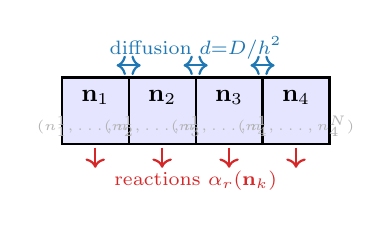
\begin{tikzpicture}[scale=0.85]
        \foreach \k in {1,2,3,4} {
          \draw[thick,fill=blue!10] (\k-1,0) rectangle (\k,1.0);
          \node[font=\small\bfseries] at (\k-0.5,0.70) {$\mathbf{n}_\k$};
          \node[font=\tiny,gray!60] at (\k-0.5,0.27)
            {$(n_\k^1,\ldots,n_\k^N)$};
        }
        \foreach \k in {1,2,3} {
          \draw[<->,fastblue,thick] (\k-0.18,1.18) -- (\k+0.18,1.18);
        }
        \node[fastblue,font=\scriptsize] at (2,1.44)
          {diffusion $d{=}D/h^2$};
        \foreach \k in {1,2,3,4} {
          \draw[->,slowred,thick] (\k-0.5,-0.05) -- (\k-0.5,-0.35);
        }
        \node[slowred,font=\scriptsize] at (2,-0.55)
          {reactions $\alpha_r(\mathbf{n}_k)$};
      \end{tikzpicture}
      \end{center}

      \smallskip
      \textbf{$\mathbf{n}_k$ is the \emph{state} of voxel $k$} — a vector, not a species label.
      \begin{itemize}\setlength\itemsep{0.2em}
        \item $N{=}1$: $\mathbf{n}_k = n_k$ (scalar)
        \item $N{>}1$: $\mathbf{n}_k\in\mathbb{Z}_{\geq 0}^N$; each voxel adds $N$ dimensions
      \end{itemize}
      The full state space is the \emph{product} of $K$ voxel state spaces.
    \end{column}
  \end{columns}

\end{frame}


\begin{frame}[shrink=5]{The RDME generator: reactions on diagonal, diffusion off-diagonal}

  \begin{columns}[T]
    \begin{column}{0.54\textwidth}
      \begin{center}
      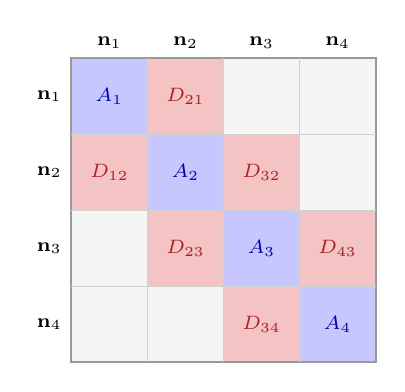
\begin{tikzpicture}[scale=0.92]
        \def\bs{1.05}
        \fill[gray!8] (0,0) rectangle (4*\bs,4*\bs);
        % Diagonal blocks: reactions A_k
        \foreach \k in {0,...,3}
          \fill[blue!22] (\k*\bs,{(3-\k)*\bs}) rectangle ({(\k+1)*\bs},{(4-\k)*\bs});
        % Off-diagonal: ALL nearest-neighbor diffusion, one color
        \fill[slowred!28] (1*\bs,3*\bs) rectangle (2*\bs,4*\bs);
        \fill[slowred!28] (0,2*\bs) rectangle (1*\bs,3*\bs);
        \fill[slowred!28] (2*\bs,2*\bs) rectangle (3*\bs,3*\bs);
        \fill[slowred!28] (1*\bs,1*\bs) rectangle (2*\bs,2*\bs);
        \fill[slowred!28] (3*\bs,1*\bs) rectangle (4*\bs,2*\bs);
        \fill[slowred!28] (2*\bs,0) rectangle (3*\bs,1*\bs);
        % Grid
        \draw[black!40,thick] (0,0) rectangle (4*\bs,4*\bs);
        \foreach \k in {1,...,3} {
          \draw[black!18,thin] (\k*\bs,0) -- (\k*\bs,4*\bs);
          \draw[black!18,thin] (0,\k*\bs) -- (4*\bs,\k*\bs);
        }
        % Block labels
        \foreach \k/\l in {0/1,1/2,2/3,3/4}
          \node[font=\scriptsize,blue!75!black]
            at ({(\k+0.5)*\bs},{(3.5-\k)*\bs}) {$A_\l$};
        \node[font=\scriptsize,slowred!80!black] at (1.5*\bs,3.5*\bs) {$D_{21}$};
        \node[font=\scriptsize,slowred!80!black] at (0.5*\bs,2.5*\bs) {$D_{12}$};
        \node[font=\scriptsize,slowred!80!black] at (2.5*\bs,2.5*\bs) {$D_{32}$};
        \node[font=\scriptsize,slowred!80!black] at (1.5*\bs,1.5*\bs) {$D_{23}$};
        \node[font=\scriptsize,slowred!80!black] at (3.5*\bs,1.5*\bs) {$D_{43}$};
        \node[font=\scriptsize,slowred!80!black] at (2.5*\bs,0.5*\bs) {$D_{34}$};
        % Axis labels: voxel states
        \foreach \k/\l in {0/$\mathbf{n}_1$,1/$\mathbf{n}_2$,2/$\mathbf{n}_3$,3/$\mathbf{n}_4$} {
          \node[above,font=\scriptsize] at ({(\k+0.5)*\bs},4*\bs) {\l};
          \node[left,font=\scriptsize]  at (0,{(3.5-\k)*\bs}) {\l};
        }
      \end{tikzpicture}
      \end{center}
      {\footnotesize $N{=}1$ shown.
      For $N{>}1$: each block is $n_{\max}^N{\times}n_{\max}^N$.
      Matrix size: $n_{\max}^{NK}{\times}n_{\max}^{NK}$.}
    \end{column}
    \begin{column}{0.42\textwidth}
      \textbf{Each axis = one voxel state $\mathbf{n}_k$.}

      \medskip
      \begin{itemize}\setlength\itemsep{0.5em}
        \item \textcolor{blue!75!black}{$A_k$}: reaction generator for voxel $k$ — diagonal block; changes $\mathbf{n}_k$ only
        \item \textcolor{slowred!80!black}{$D_{k,k+1}$}: diffusion coupling — off-diagonal, nearest-neighbor; changes $\mathbf{n}_k$ and $\mathbf{n}_{k+1}$
      \end{itemize}

      \medskip
      $A = A_\mathrm{rxn} + A_\mathrm{diff}$, block-tridiagonal.

      \medskip
      Sparse: each transition changes at most two neighboring voxel states.

      \medskip
      \begin{alertblock}{The challenge}
        Size $n_{\max}^{NK}$ explodes as $K$ grows.
        \textbf{Goal:} reduce without losing accuracy.
      \end{alertblock}
    \end{column}
  \end{columns}

\end{frame}


% ================================================================
\section{How Grouping Works}
% ================================================================

\begin{frame}[shrink=15]{Coarsening a voxel pair: restriction and Binomial split-back}

  Pair $(n_1,n_2)$: diffusion conserves the total $\bar n = n_1{+}n_2$.
  \textit{Shown for $S{=}1$, $m{=}2$; extends to any $S$, $m$ by independence of species.}

  \begin{columns}[T]
    \begin{column}{0.44\textwidth}
      \begin{block}{Marginalize ($\calR$) — exact}
        \vspace{-0.5em}
        \[ p^c\!\bigl((\bar n_s)_s\bigr) =
           \!\!\!\sum_{\substack{\text{configs}\\\text{with totals }(\bar n_s)}}\!\!\! p(\ldots). \]
        \vspace{-0.8em}
      \end{block}

      \begin{block}{Split back ($\calP$) — independent per species}
        \vspace{-0.3em}
        \[ \calP = \prod_{s=1}^S \Bin\!\bigl(\bar n_s,\tfrac{1}{m}\bigr). \]
        \vspace{-0.4em}
        ($m{=}2$: Binomial; $m{>}2$: Multinomial.)\\
        Valid when diffusion dominates within the group.
      \end{block}

      \begin{block}{State-space reduction}
        \vspace{-0.2em}
        Per group: $n_{\max}^{mS} \!\to\! n_{\max}^{S}$.\\[0.1em]
        $K/m$ groups all coarse: $n_{\max}^{KS} \!\to\! n_{\max}^{KS/m}$.
      \end{block}
    \end{column}
    \begin{column}{0.20\textwidth}
      \vspace{1.2cm}
      \begin{center}
      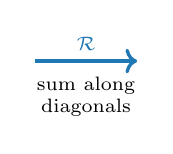
\begin{tikzpicture}
        \draw[->,very thick,coarsecolor] (0,0.3) -- (1.3,0.3)
          node[above,midway,font=\scriptsize]{$\calR$};
        \node[font=\scriptsize,align=center] at (0.65,-0.15) {sum along\\diagonals};
      \end{tikzpicture}

      \vspace{0.7cm}
      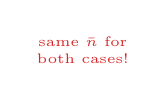
\begin{tikzpicture}
        \node[font=\tiny,align=center,slowred] at (0.65,0.3)
          {same $\bar n$ for\\both cases!};
      \end{tikzpicture}

      \vspace{0.5cm}
      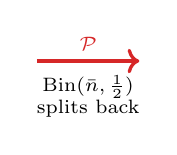
\begin{tikzpicture}
        \draw[->,very thick,slowred] (0,0.3) -- (1.3,0.3)
          node[above,midway,font=\scriptsize]{$\calP$};
        \node[font=\scriptsize,align=center] at (0.65,-0.15) {$\Bin(\bar n,\frac{1}{2})$\\splits back};
      \end{tikzpicture}
      \end{center}
    \end{column}
    \begin{column}{0.32\textwidth}
      \textit{Uniform — $\calP(\calR\,p)\approx p$.} \textcolor{coarsegreen!80!black}{\checkmark}

      \begin{center}
      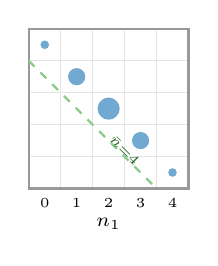
\begin{tikzpicture}[scale=0.78]
        \def\cs{0.52}
        \draw[gray!20](0,0) grid[step=\cs] (5*\cs,5*\cs);
        \draw[black!40,thick](0,0) rectangle (5*\cs,5*\cs);
        \draw[coarsegreen!55,dashed,thick](0,4*\cs)--(4*\cs,0);
        \node[coarsegreen!60!black,font=\tiny,rotate=-45] at (3.0*\cs,1.2*\cs){$\bar n{=}4$};
        \fill[coarsecolor!70,opacity=0.9](0.26,2.34) circle (0.07cm);
        \fill[coarsecolor!70,opacity=0.9](0.78,1.82) circle (0.14cm);
        \fill[coarsecolor!70,opacity=0.9](1.30,1.30) circle (0.18cm);
        \fill[coarsecolor!70,opacity=0.9](1.82,0.78) circle (0.14cm);
        \fill[coarsecolor!70,opacity=0.9](2.34,0.26) circle (0.07cm);
        \foreach \n in {0,1,2,3,4}
          \node[below,font=\tiny] at ({(\n+0.5)*\cs},0) {\n};
        \node[below,font=\scriptsize] at (1.3,{-0.32}) {$n_1$};
      \end{tikzpicture}
      \end{center}

      \vspace{0.3em}
      \textit{Front — Binomial peaks at centre; true is bimodal.} \textcolor{slowred}{\ding{55}}

      \begin{center}
      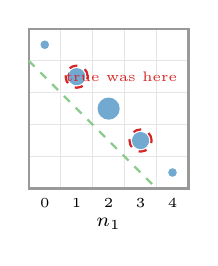
\begin{tikzpicture}[scale=0.78]
        \def\cs{0.52}
        \draw[gray!20](0,0) grid[step=\cs] (5*\cs,5*\cs);
        \draw[black!40,thick](0,0) rectangle (5*\cs,5*\cs);
        \draw[coarsegreen!55,dashed,thick](0,4*\cs)--(4*\cs,0);
        \fill[coarsecolor!70,opacity=0.9](0.26,2.34) circle (0.07cm);
        \fill[coarsecolor!70,opacity=0.9](0.78,1.82) circle (0.14cm);
        \fill[coarsecolor!70,opacity=0.9](1.30,1.30) circle (0.18cm);
        \fill[coarsecolor!70,opacity=0.9](1.82,0.78) circle (0.14cm);
        \fill[coarsecolor!70,opacity=0.9](2.34,0.26) circle (0.07cm);
        \draw[slowred,thick,dashed](0.78,1.82) circle (0.18cm);
        \draw[slowred,thick,dashed](1.82,0.78) circle (0.18cm);
        \node[slowred,font=\tiny] at (2.9*\cs,3.5*\cs){true was here};
        \foreach \n in {0,1,2,3,4}
          \node[below,font=\tiny] at ({(\n+0.5)*\cs},0) {\n};
        \node[below,font=\scriptsize] at (1.3,{-0.32}) {$n_1$};
      \end{tikzpicture}
      \end{center}
      {\tiny Reconstructed (\textcolor{coarsecolor}{filled}) vs.\ true (\textcolor{slowred}{dashed}).}
    \end{column}
  \end{columns}

\end{frame}


\begin{frame}[shrink=5]{Why the Binomial: diffusion alone equilibrates to $\Bin(\bar n,\,\tfrac{1}{2})$}

  Fix total $\bar n = n_1 + n_2$.
  Within-group diffusion alone is a birth-death chain on $\{0,\ldots,\bar n\}$:

  \begin{center}
  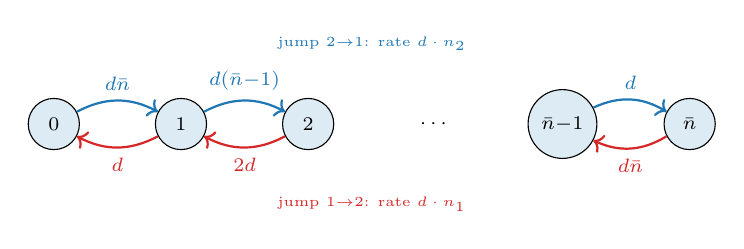
\begin{tikzpicture}[every node/.style={font=\scriptsize}, scale=0.85]
    \node[draw,circle,minimum size=0.65cm,fill=coarsecolor!15] (s0) at (0,    0) {$0$};
    \node[draw,circle,minimum size=0.65cm,fill=coarsecolor!15] (s1) at (1.9,  0) {$1$};
    \node[draw,circle,minimum size=0.65cm,fill=coarsecolor!15] (s2) at (3.8,  0) {$2$};
    \node at (5.7, 0) {$\cdots$};
    \node[draw,circle,minimum size=0.80cm,fill=coarsecolor!15] (s4) at (7.6,  0) {$\bar n{-}1$};
    \node[draw,circle,minimum size=0.65cm,fill=coarsecolor!15] (s5) at (9.5,  0) {$\bar n$};
    \draw[->,fastblue,thick,bend left=28] (s0) to node[above]{$d\bar n$}          (s1);
    \draw[->,fastblue,thick,bend left=28] (s1) to node[above]{$d(\bar n{-}1)$}   (s2);
    \draw[->,fastblue,thick,bend left=28] (s4) to node[above]{$d$}                (s5);
    \draw[->,slowred, thick,bend left=28] (s1) to node[below]{$d$}                (s0);
    \draw[->,slowred, thick,bend left=28] (s2) to node[below]{$2d$}               (s1);
    \draw[->,slowred, thick,bend left=28] (s5) to node[below]{$d\bar n$}          (s4);
    \node[fastblue,above,font=\tiny] at (4.75,0.95) {jump $2{\to}1$: rate $d\cdot n_2$};
    \node[slowred, below,font=\tiny] at (4.75,-0.95) {jump $1{\to}2$: rate $d\cdot n_1$};
  \end{tikzpicture}
  \end{center}

  \begin{columns}[T]
    \begin{column}{0.50\textwidth}
      \textbf{Detailed balance:}
      \[
        \pi(n_1)\cdot d(\bar n - n_1) \;=\; \pi(n_1{+}1)\cdot d(n_1{+}1)
      \]
      \[
        \frac{\pi(n_1{+}1)}{\pi(n_1)}
        = \frac{\bar n - n_1}{n_1{+}1}
        = \frac{\tbinom{\bar n}{n_1+1}}{\tbinom{\bar n}{n_1}}
      \]
      \[
        \boxed{\pi(n_1) = \Bin\!\bigl(\bar n,\,\tfrac{1}{2}\bigr)} \quad \textbf{(exact)}
      \]
    \end{column}
    \begin{column}{0.46\textwidth}
      \begin{block}{Exact vs.\ approximate}
        \textbf{Exact:} $\Bin(\bar n,\tfrac12)$ is the stationary distribution
        for any $d>0$.\\[0.3em]
        \textbf{Approximate:} valid when $d_s \gg \alpha_r$ for all species $s$.\\[0.3em]
        \textbf{$S>1$:} one independent chain per species; joint prolongation
        $= \prod_s \Bin(\bar n_s, 1/m)$.\\[0.3em]
        \textbf{$m>2$:} $\Bin \to \text{Mult}(\bar n_s;\,1/m,\ldots,1/m)$.
      \end{block}
    \end{column}
  \end{columns}

\end{frame}


\begin{frame}[shrink=8]{What grouping does to the generator}

  \begin{columns}[T]
    \begin{column}{0.43\textwidth}
      \textbf{Full-resolution generator $A$ — 4 voxels:}

      \begin{center}
      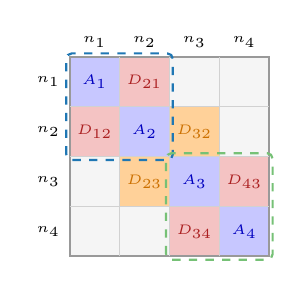
\begin{tikzpicture}[scale=0.72]
        \def\bs{0.88}
        \fill[gray!8] (0,0) rectangle (4*\bs,4*\bs);
        \foreach \k in {0,...,3}
          \fill[blue!22] (\k*\bs,{(3-\k)*\bs}) rectangle ({(\k+1)*\bs},{(4-\k)*\bs});
        \fill[slowred!28] (1*\bs,3*\bs) rectangle (2*\bs,4*\bs);
        \fill[slowred!28] (0,2*\bs) rectangle (1*\bs,3*\bs);
        \fill[slowred!28] (3*\bs,1*\bs) rectangle (4*\bs,2*\bs);
        \fill[slowred!28] (2*\bs,0) rectangle (3*\bs,1*\bs);
        \fill[intercolor!40] (2*\bs,2*\bs) rectangle (3*\bs,3*\bs);
        \fill[intercolor!40] (1*\bs,1*\bs) rectangle (2*\bs,2*\bs);
        \draw[black!40,thick] (0,0) rectangle (4*\bs,4*\bs);
        \foreach \k in {1,...,3} {
          \draw[black!18,thin] (\k*\bs,0) -- (\k*\bs,4*\bs);
          \draw[black!18,thin] (0,\k*\bs) -- (4*\bs,\k*\bs);
        }
        \draw[coarsecolor,thick,dashed,rounded corners=2pt]
          (-0.06,2*\bs-0.06) rectangle (2*\bs+0.06,4*\bs+0.06);
        \draw[coarsegreen!65,thick,dashed,rounded corners=2pt]
          (2*\bs-0.06,-0.06) rectangle (4*\bs+0.06,2*\bs+0.06);
        \foreach \k/\l in {0/1,1/2,2/3,3/4}
          \node[font=\tiny,blue!75!black] at ({(\k+0.5)*\bs},{(3.5-\k)*\bs}) {$A_\l$};
        \node[font=\tiny,slowred!80!black] at (1.5*\bs,3.5*\bs) {$D_{21}$};
        \node[font=\tiny,slowred!80!black] at (0.5*\bs,2.5*\bs) {$D_{12}$};
        \node[font=\tiny,slowred!80!black] at (3.5*\bs,1.5*\bs) {$D_{43}$};
        \node[font=\tiny,slowred!80!black] at (2.5*\bs,0.5*\bs) {$D_{34}$};
        \node[font=\tiny,intercolor!80!black] at (2.5*\bs,2.5*\bs) {$D_{32}$};
        \node[font=\tiny,intercolor!80!black] at (1.5*\bs,1.5*\bs) {$D_{23}$};
        \foreach \k/\l in {0/$n_1$,1/$n_2$,2/$n_3$,3/$n_4$} {
          \node[above,font=\tiny] at ({(\k+0.5)*\bs},4*\bs) {\l};
          \node[left,font=\tiny]  at (0,{(3.5-\k)*\bs}) {\l};
        }
      \end{tikzpicture}
      \end{center}
      {\footnotesize State space: $n_{\max}^4$}
    \end{column}
    \begin{column}{0.12\textwidth}
      \vspace{2.8cm}
      \begin{center}
        $\xrightarrow{\;\calR\;}$\\[0.5em]
        $\xleftarrow{\;\calP\;}$
      \end{center}
    \end{column}
    \begin{column}{0.42\textwidth}
      \textbf{Coarse generator $\bar A$ — 2 groups:}

      \begin{center}
      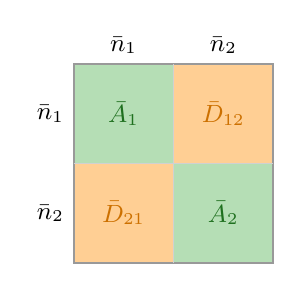
\begin{tikzpicture}[scale=0.72]
        \def\cs{1.76}
        \fill[gray!8] (0,0) rectangle (2*\cs,2*\cs);
        \fill[coarsegreen!35] (0,\cs) rectangle (\cs,2*\cs);
        \fill[coarsegreen!35] (\cs,0) rectangle (2*\cs,\cs);
        \fill[intercolor!42] (0,0) rectangle (\cs,\cs);
        \fill[intercolor!42] (\cs,\cs) rectangle (2*\cs,2*\cs);
        \draw[black!40,thick] (0,0) rectangle (2*\cs,2*\cs);
        \draw[black!18,thin] (\cs,0) -- (\cs,2*\cs);
        \draw[black!18,thin] (0,\cs) -- (2*\cs,\cs);
        \node[font=\small,coarsegreen!70!black] at (0.5*\cs,1.5*\cs) {$\bar A_1$};
        \node[font=\small,coarsegreen!70!black] at (1.5*\cs,0.5*\cs) {$\bar A_2$};
        \node[font=\small,intercolor!80!black]  at (0.5*\cs,0.5*\cs) {$\bar D_{21}$};
        \node[font=\small,intercolor!80!black]  at (1.5*\cs,1.5*\cs) {$\bar D_{12}$};
        \node[above,font=\small] at (0.5*\cs,2*\cs) {$\bar n_1$};
        \node[above,font=\small] at (1.5*\cs,2*\cs) {$\bar n_2$};
        \node[left,font=\small]  at (0,1.5*\cs) {$\bar n_1$};
        \node[left,font=\small]  at (0,0.5*\cs) {$\bar n_2$};
      \end{tikzpicture}
      \end{center}
      {\footnotesize State space: $n_{\max}^2$ \quad ($K{=}8{\to}4$: \textbf{$3{\times}10^4$ smaller})}

      \smallskip
      \begin{itemize}\setlength\itemsep{0.3em}
        \item \textcolor{slowred!80!black}{$D_{12},D_{21}$} \textbf{disappear} — diffusion inside each group is absorbed into the Binomial
        \item \textcolor{coarsegreen!70!black}{$\bar A_j = \calR(A_{2j-1}+A_{2j})\calP$} — Binomial-averaged reactions for pair $j$
        \item \textcolor{intercolor!80!black}{$\bar D_{23}$} — diffusion at the group boundary (rescaled by $\calR,\calP$)
      \end{itemize}
    \end{column}
  \end{columns}

\end{frame}


% ================================================================
\section{Grouping Fails When\ldots}
% ================================================================


\begin{frame}[shrink=4]{Numerical example: Schl\"ogl model ($S{=}1$, $m{=}2$, $K{=}8$)}

  \begin{columns}[T]
    \begin{column}{0.44\textwidth}
      \textbf{Schl\"ogl model:} each voxel has two stable molecule counts.

      \begin{block}{Single-voxel fixed points}
        $n_{\mathrm{low}}=31,\quad n_{\mathrm{barrier}}=72,\quad n_{\mathrm{high}}=162.$
      \end{block}

      \medskip
      A \textbf{front} forms when neighboring voxels settle in opposite stable states.
      The interface drifts stochastically along the domain.

      \medskip
      Diffusion rate $d{=}D/h^2{=}0.08$ — slow relative to bistable reactions,
      which sustains the front indefinitely.
    \end{column}
    \begin{column}{0.52\textwidth}
      \begin{center}
      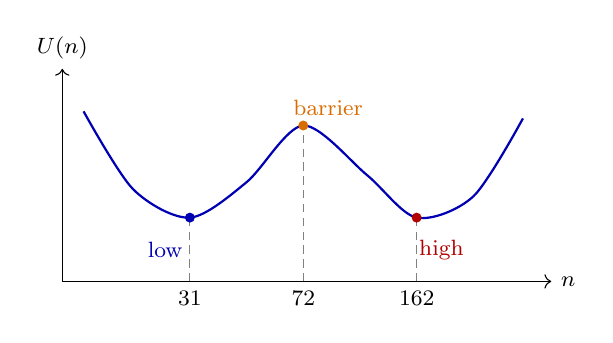
\begin{tikzpicture}[scale=0.90, every node/.style={font=\footnotesize}]
        \draw[->] (0,0) -- (6.9,0) node[right] {$n$};
        \draw[->] (0,0) -- (0,3.0) node[above] {$U(n)$};
        \draw[thick,blue!70!black]
          plot[smooth] coordinates {(0.3,2.4)(1.0,1.3)(1.8,0.9)(2.6,1.4)
                                    (3.4,2.2)(4.3,1.5)(5.0,0.9)(5.8,1.2)(6.5,2.3)};
        \draw[densely dashed,gray] (1.8,0) -- (1.8,0.9);
        \draw[densely dashed,gray] (3.4,0) -- (3.4,2.2);
        \draw[densely dashed,gray] (5.0,0) -- (5.0,0.9);
        \fill[blue!70!black] (1.8,0.9) circle (2pt);
        \fill[orange!85!black] (3.4,2.2) circle (2pt);
        \fill[red!70!black] (5.0,0.9) circle (2pt);
        \node[below] at (1.8,0) {$31$};
        \node[below] at (3.4,0) {$72$};
        \node[below] at (5.0,0) {$162$};
        \node[blue!70!black] at (1.45,0.45) {low};
        \node[orange!85!black] at (3.75,2.45) {barrier};
        \node[red!70!black] at (5.35,0.45) {high};
      \end{tikzpicture}

      \medskip
      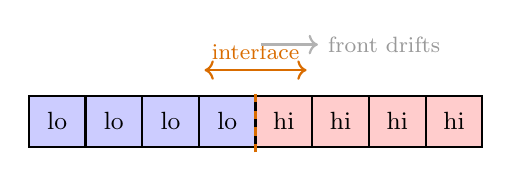
\begin{tikzpicture}[scale=0.72]
        \foreach \k in {1,2,3,4} {
          \draw[thick,fill=blue!20] (\k-1,0) rectangle (\k,0.9);
          \node[font=\small] at (\k-0.5,0.45) {lo};
        }
        \foreach \k in {5,6,7,8} {
          \draw[thick,fill=red!20] (\k-1,0) rectangle (\k,0.9);
          \node[font=\small] at (\k-0.5,0.45) {hi};
        }
        \draw[very thick,orange!85!black,dashed] (4,-0.1) -- (4,1.05);
        \draw[<->,thick,orange!85!black] (3.1,1.35) -- (4.9,1.35)
          node[midway,above,font=\footnotesize]{interface};
        \draw[->,thick,gray!60] (4.1,1.8) -- (5.1,1.8)
          node[right,font=\footnotesize,gray!80]{front drifts};
      \end{tikzpicture}
      \end{center}
    \end{column}
  \end{columns}

\end{frame}


\begin{frame}[shrink=3]{The Binomial approximation fails at the front}

  \begin{center}
    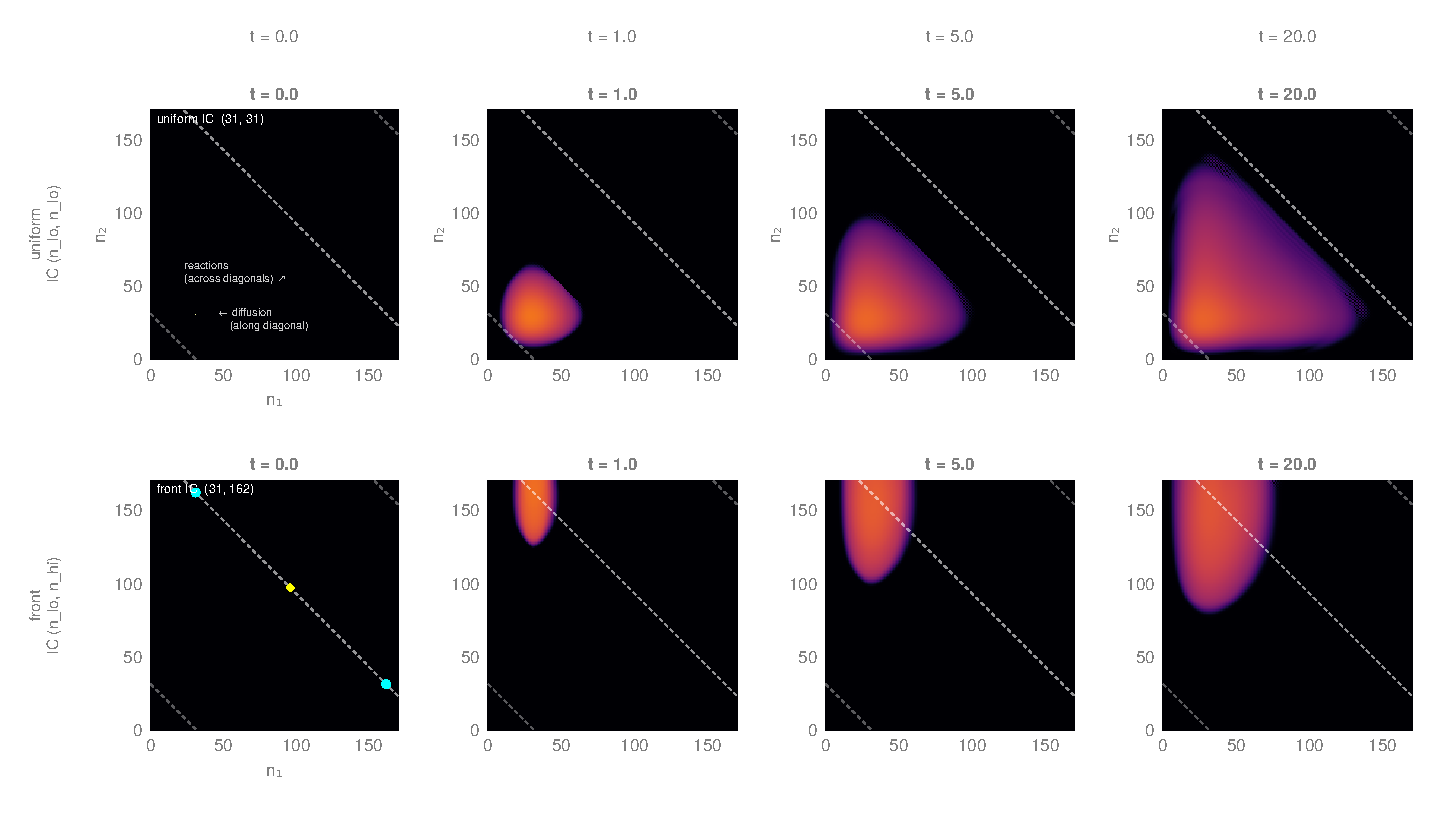
\includegraphics[width=\textwidth,height=0.68\textheight,keepaspectratio]{fig_prob_diffusion}
  \end{center}

  {\footnotesize
  K=2 Schl\"ogl ($D=0.005$, $d=0.02$).
  \textbf{Top (uniform, $(31,31)$):} diffusion moves probability along constant-total lines;
  conditional $\to\Bin(\bar n,\tfrac12)$ — grouping is valid.
  \textbf{Bottom (front, $(31,162)$):} bistable reactions outrun diffusion; probability stays
  at the corners; conditional $\ne\Bin(\bar n,\tfrac12)$ — grouping is invalid.
  Dashed diagonals $=$ constant-total lines.}

\end{frame}


\begin{frame}[shrink=5]{The imbalance criterion $\alpha_j$}

  \begin{columns}[T]
    \begin{column}{0.50\textwidth}
      Per-species imbalance within group $j$:
      \[
        \alpha_{j,s} = \frac{|\mu_{2j-1,s} - \mu_{2j,s}|}{\mu_{2j-1,s}+\mu_{2j,s}},
        \qquad
        \alpha_j = \max_s\,\alpha_{j,s}.
      \]
      Small $\alpha_j$: all species balanced — diffusion dominates within the group.

      \medskip
      \begin{block}{The coarsening rule}
        \textbf{Coarsen group $j$ iff $\alpha_j < \alpha_{\rm lo}$.}\\[0.3em]
        \begin{itemize}
          \item Non-equilibrium IC: $\alpha_j$ starts large, decays as diffusion acts
          \item Bistable front: $\alpha_j$ stays large (reactions as fast as diffusion)
        \end{itemize}
        Split-back applied only where diffusion dominates for all species.
      \end{block}
    \end{column}
    \begin{column}{0.46\textwidth}
      \begin{center}
        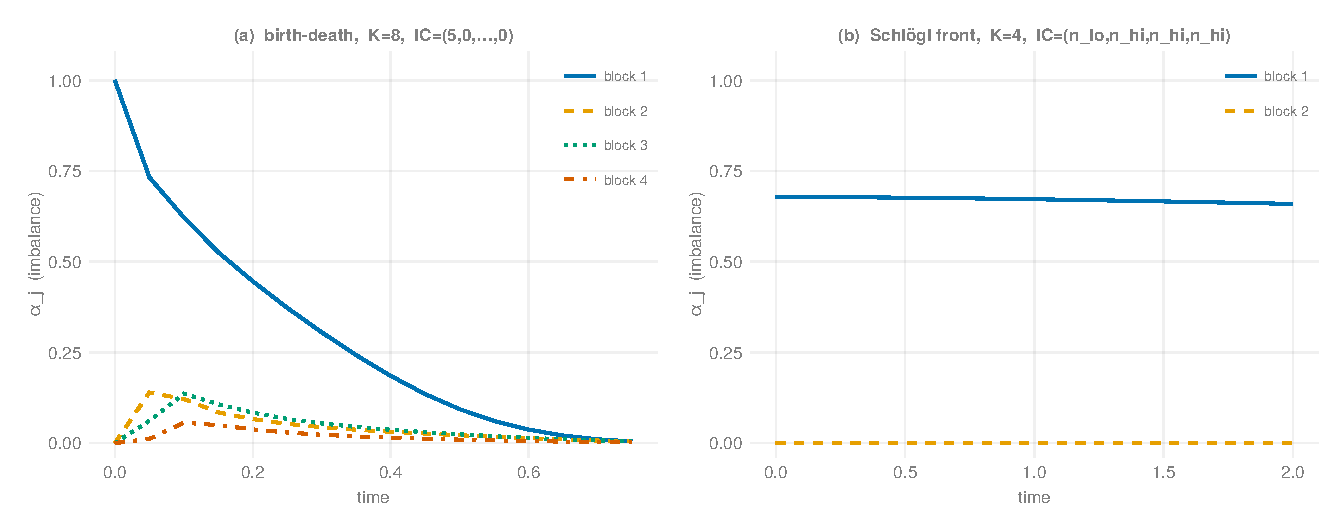
\includegraphics[width=\textwidth,height=0.60\textheight,keepaspectratio]{fig_criterion}
      \end{center}
      {\footnotesize
      \textbf{(a)} Birth-death: $\alpha_1$ decays to zero (diffusion equilibrates the pair).
      \textbf{(b)} Schl\"ogl front: $\alpha_1$ persists (bistable reactions outrun diffusion).
      Green band = region where grouping is valid.}
    \end{column}
  \end{columns}

\end{frame}


\begin{frame}{Adaptive grouping eliminates the error}

  \begin{center}
    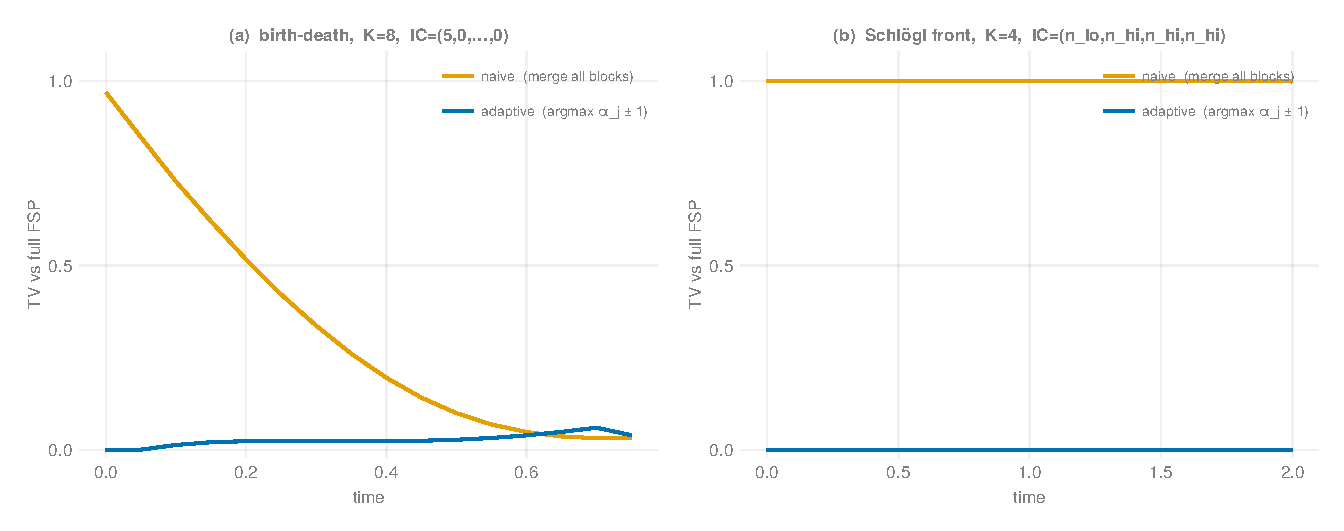
\includegraphics[width=\textwidth,height=0.62\textheight,keepaspectratio]{fig_tv_criterion}
  \end{center}

  {\footnotesize
  \textbf{(a)} Birth-death: uniform coarsening (Binomial from $t{=}0$) gives TV${=}0.97$ immediately.
  Adaptive (coarsen only when $\alpha{<}\alpha_{\rm lo}$): TV${=}0$ until equilibration, then small.
  \textbf{(b)} Schl\"ogl front: uniform coarsening gives TV${=}1.0$ throughout (orientation destroyed).
  Adaptive (keep group 1 at fine resolution): TV${=}0$ throughout.}

\end{frame}


% ================================================================
\section{The Adaptive Algorithm}
% ================================================================


\begin{frame}{The mixed-resolution RDME}

  Replace $(n_{2j-1},n_{2j})$ by the total $\bar n_j$ for equilibrated pairs;
  keep front pairs at full resolution.

  \begin{center}
  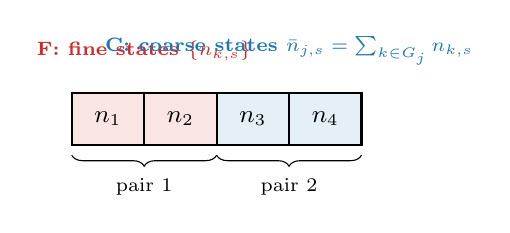
\begin{tikzpicture}[scale=0.92, every node/.style={font=\small}]
    % Labels above — well separated
    \node[slowred,font=\scriptsize\bfseries] at (1, 1.30)
      {\textbf{F}: fine states $\{n_{k,s}\}$};
    \node[coarsecolor,font=\scriptsize\bfseries] at (3, 1.30)
      {\textbf{C}: coarse states $\bar n_{j,s} = \sum_{k\in G_j} n_{k,s}$};
    % Voxels
    \foreach \k in {1,2} {
      \draw[thick,fill=slowred!12] (\k-1,0) rectangle (\k,0.72);
      \node at (\k-0.5,0.36) {$n_\k$};
    }
    \foreach \k in {3,4} {
      \draw[thick,fill=coarsecolor!12] (\k-1,0) rectangle (\k,0.72);
      \node at (\k-0.5,0.36) {$n_\k$};
    }
    % Braces
    \draw[decorate,decoration={brace,mirror,amplitude=4pt}]
      (0,-0.14) -- (2,-0.14) node[midway,below=5pt,font=\scriptsize]{pair 1};
    \draw[decorate,decoration={brace,mirror,amplitude=4pt}]
      (2,-0.14) -- (4,-0.14) node[midway,below=5pt,font=\scriptsize]{pair 2};
  \end{tikzpicture}
  \end{center}

  \begin{columns}[T]
    \begin{column}{0.52\textwidth}
      \begin{itemize}\setlength\itemsep{0.5em}
        \item \textbf{Fine (F):} full joint distribution $\{n_{k,s}\}_{k\in G_j}$; within-group diffusion tracked exactly
        \item \textbf{Coarse (C):} only totals $(\bar n_{j,s})_s$; within-group diffusion absorbed into $\prod_s\Bin(\bar n_{j,s},\tfrac{1}{m})$
        \item \textbf{Evolve directly:} $\dot p^M = A^M p^M$ — no convert-back step
      \end{itemize}
    \end{column}
    \begin{column}{0.44\textwidth}
      \begin{block}{State-space savings}
        Per group: $n_{\max}^{mS}$ fine $\to$ $n_{\max}^S$ coarse.\\[0.2em]
        $K/m$ groups all coarse: $n_{\max}^{KS}\to n_{\max}^{KS/m}$.
      \end{block}
      \smallskip
      {\small Coarsen where $\alpha_j < \alpha_{\rm lo}$; keep fine near the front.}
    \end{column}
  \end{columns}

\end{frame}


\begin{frame}[shrink=4]{Tracking the drifting front}

  \begin{center}
  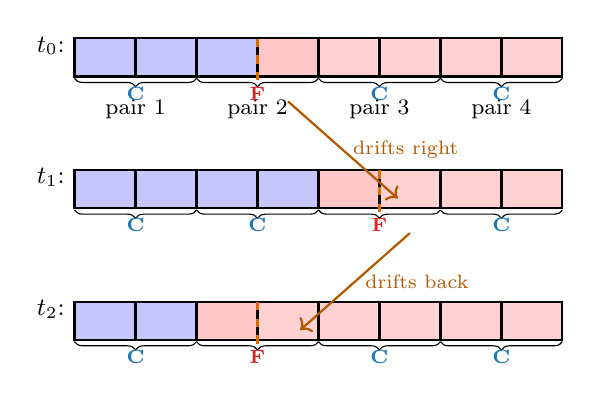
\begin{tikzpicture}[scale=0.88, every node/.style={font=\footnotesize}]
    \def\vh{0.55}
    \def\vw{0.88}

    % ── Row 1: t = t_0 ───────────────────────────────────────────────────────
    \node[left,font=\small] at (0, 1.8*\vh) {$t_0$:};
    \foreach \k/\col in {1/blue!22,2/blue!22,3/blue!22,4/red!22,5/red!18,6/red!18,7/red!18,8/red!18} {
      \draw[thick,fill=\col] ({(\k-1)*\vw},\vh) rectangle ({\k*\vw},{2*\vh});
    }
    \foreach \j/\xl/\xr/\lbl in {1/0/2/1, 2/2/4/2, 3/4/6/3, 4/6/8/4} {
      \draw[decorate,decoration={brace,mirror,amplitude=3pt}]
        ({\xl*\vw},0.95*\vh) -- ({\xr*\vw},0.95*\vh)
        node[midway,below=4pt]{pair \lbl};
    }
    \node[coarsecolor,font=\scriptsize\bfseries] at ({1*\vw},0.55*\vh) {C};
    \node[slowred,font=\scriptsize\bfseries]     at ({3*\vw},0.55*\vh) {F};
    \node[coarsecolor,font=\scriptsize\bfseries] at ({5*\vw},0.55*\vh) {C};
    \node[coarsecolor,font=\scriptsize\bfseries] at ({7*\vw},0.55*\vh) {C};
    \draw[very thick,orange!85!black,dashed] ({3*\vw},0.9*\vh) -- ({3*\vw},{2.1*\vh});

    % ── Row 2: t = t_1 ───────────────────────────────────────────────────────
    \node[left,font=\small] at (0, 1.8*\vh - 1.9) {$t_1$:};
    \foreach \k/\col in {1/blue!22,2/blue!22,3/blue!22,4/blue!22,5/red!22,6/red!18,7/red!18,8/red!18} {
      \draw[thick,fill=\col] ({(\k-1)*\vw},\vh-1.9) rectangle ({\k*\vw},{2*\vh-1.9});
    }
    \foreach \j/\xl/\xr/\lbl in {1/0/2/1, 2/2/4/2, 3/4/6/3, 4/6/8/4} {
      \draw[decorate,decoration={brace,mirror,amplitude=3pt}]
        ({\xl*\vw},0.95*\vh-1.9) -- ({\xr*\vw},0.95*\vh-1.9)
        node[midway,below=4pt]{};
    }
    \node[coarsecolor,font=\scriptsize\bfseries] at ({1*\vw},0.55*\vh-1.9) {C};
    \node[coarsecolor,font=\scriptsize\bfseries] at ({3*\vw},0.55*\vh-1.9) {C};
    \node[slowred,font=\scriptsize\bfseries]     at ({5*\vw},0.55*\vh-1.9) {F};
    \node[coarsecolor,font=\scriptsize\bfseries] at ({7*\vw},0.55*\vh-1.9) {C};
    \draw[very thick,orange!85!black,dashed] ({5*\vw},0.9*\vh-1.9) -- ({5*\vw},{2.1*\vh-1.9});

    % ── Row 3: t = t_2 ───────────────────────────────────────────────────────
    \node[left,font=\small] at (0, 1.8*\vh - 3.8) {$t_2$:};
    \foreach \k/\col in {1/blue!22,2/blue!22,3/red!22,4/red!18,5/red!18,6/red!18,7/red!18,8/red!18} {
      \draw[thick,fill=\col] ({(\k-1)*\vw},\vh-3.8) rectangle ({\k*\vw},{2*\vh-3.8});
    }
    \foreach \j/\xl/\xr/\lbl in {1/0/2/1, 2/2/4/2, 3/4/6/3, 4/6/8/4} {
      \draw[decorate,decoration={brace,mirror,amplitude=3pt}]
        ({\xl*\vw},0.95*\vh-3.8) -- ({\xr*\vw},0.95*\vh-3.8)
        node[midway,below=4pt]{};
    }
    \node[coarsecolor,font=\scriptsize\bfseries] at ({1*\vw},0.55*\vh-3.8) {C};
    \node[slowred,font=\scriptsize\bfseries]     at ({3*\vw},0.55*\vh-3.8) {F};
    \node[coarsecolor,font=\scriptsize\bfseries] at ({5*\vw},0.55*\vh-3.8) {C};
    \node[coarsecolor,font=\scriptsize\bfseries] at ({7*\vw},0.55*\vh-3.8) {C};
    \draw[very thick,orange!85!black,dashed] ({3*\vw},0.9*\vh-3.8) -- ({3*\vw},{2.1*\vh-3.8});

    % Drift arrows between rows
    \draw[->,thick,orange!70!black] ({3.5*\vw},0.8*\vh-0.25) -- ({5.3*\vw},0.8*\vh-1.65)
      node[midway,right,font=\scriptsize]{drifts right};
    \draw[->,thick,orange!70!black] ({5.5*\vw},0.8*\vh-2.15) -- ({3.7*\vw},0.8*\vh-3.55)
      node[midway,right,font=\scriptsize]{drifts back};
  \end{tikzpicture}
  \end{center}

  \smallskip
  {\small The fine window (\textcolor{slowred}{\textbf{F}}) keeps the front pair at full resolution.
  Groups far from the front (\textcolor{coarsecolor}{\textbf{C}} = coarse) stay coarse.
  Resolution is updated only when the front crosses a pair boundary.}

\end{frame}


\begin{frame}[shrink=14]{The mixed-resolution generator}

  \begin{columns}[T]
    \begin{column}{0.46\textwidth}
      \textbf{Full-resolution generator $A$ ($K=4$):}

      \begin{center}
      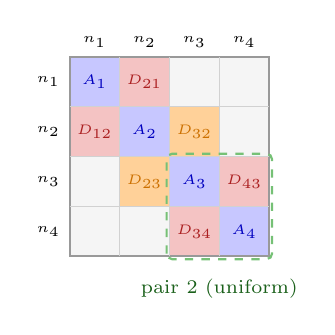
\begin{tikzpicture}[scale=0.72]
        \def\bs{0.88}
        \fill[gray!8] (0,0) rectangle (4*\bs,4*\bs);
        \foreach \k in {0,...,3}
          \fill[blue!22] (\k*\bs,{(3-\k)*\bs}) rectangle ({(\k+1)*\bs},{(4-\k)*\bs});
        \fill[slowred!28] (1*\bs,3*\bs) rectangle (2*\bs,4*\bs);
        \fill[slowred!28] (0,2*\bs) rectangle (1*\bs,3*\bs);
        \fill[slowred!28] (3*\bs,1*\bs) rectangle (4*\bs,2*\bs);
        \fill[slowred!28] (2*\bs,0) rectangle (3*\bs,1*\bs);
        \fill[intercolor!40] (2*\bs,2*\bs) rectangle (3*\bs,3*\bs);
        \fill[intercolor!40] (1*\bs,1*\bs) rectangle (2*\bs,2*\bs);
        \draw[black!40,thick] (0,0) rectangle (4*\bs,4*\bs);
        \foreach \k in {1,...,3} {
          \draw[black!18,thin] (\k*\bs,0) -- (\k*\bs,4*\bs);
          \draw[black!18,thin] (0,\k*\bs) -- (4*\bs,\k*\bs);
        }
        \draw[coarsegreen!65,thick,dashed,rounded corners=2pt]
          (2*\bs-0.05,-0.05) rectangle (4*\bs+0.05,2*\bs+0.05);
        \foreach \k/\l in {0/1,1/2,2/3,3/4}
          \node[font=\tiny,blue!75!black] at ({(\k+0.5)*\bs},{(3.5-\k)*\bs}) {$A_\l$};
        \node[font=\tiny,slowred!80!black] at (1.5*\bs,3.5*\bs) {$D_{21}$};
        \node[font=\tiny,slowred!80!black] at (0.5*\bs,2.5*\bs) {$D_{12}$};
        \node[font=\tiny,slowred!80!black] at (3.5*\bs,1.5*\bs) {$D_{43}$};
        \node[font=\tiny,slowred!80!black] at (2.5*\bs,0.5*\bs) {$D_{34}$};
        \node[font=\tiny,intercolor!80!black] at (2.5*\bs,2.5*\bs) {$D_{32}$};
        \node[font=\tiny,intercolor!80!black] at (1.5*\bs,1.5*\bs) {$D_{23}$};
        \foreach \k/\l in {0/$n_1$,1/$n_2$,2/$n_3$,3/$n_4$} {
          \node[above,font=\tiny] at ({(\k+0.5)*\bs},4*\bs) {\l};
          \node[left,font=\tiny]  at (0,{(3.5-\k)*\bs}) {\l};
        }
        \node[coarsegreen!60!black,font=\scriptsize,below] at (3*\bs,-0.22) {pair 2 (uniform)};
      \end{tikzpicture}
      \end{center}
    \end{column}
    \begin{column}{0.50\textwidth}
      \textbf{Mixed generator $A^M$ (pair 2 grouped):}

      \begin{center}
      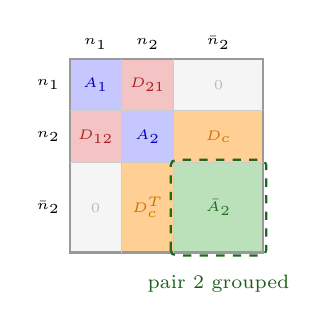
\begin{tikzpicture}[scale=0.75]
        \def\f{0.88}
        \def\c{1.52}
        \fill[gray!8] (0,0) rectangle (2*\f+\c, 2*\f+\c);
        \fill[blue!22]        (0,\f+\c) rectangle (\f,2*\f+\c);
        \fill[blue!22]        (\f,\c)   rectangle (2*\f,\f+\c);
        \fill[coarsegreen!32] (2*\f,0)  rectangle (2*\f+\c,\c);
        \fill[slowred!28] (\f,\f+\c) rectangle (2*\f,2*\f+\c);
        \fill[slowred!28] (0,\c)     rectangle (\f,\f+\c);
        \fill[intercolor!42] (2*\f,\c) rectangle (2*\f+\c,\f+\c);
        \fill[intercolor!42] (\f,0)    rectangle (2*\f,\c);
        \draw[black!40,thick] (0,0) rectangle (2*\f+\c, 2*\f+\c);
        \draw[black!20,thin] (\f,0)   -- (\f,2*\f+\c);
        \draw[black!20,thin] (2*\f,0) -- (2*\f,2*\f+\c);
        \draw[black!20,thin] (0,\c)   -- (2*\f+\c,\c);
        \draw[black!20,thin] (0,\f+\c) -- (2*\f+\c,\f+\c);
        \draw[coarsegreen!65!black,thick,dashed,rounded corners=2pt]
          (2*\f-0.05,-0.05) rectangle (2*\f+\c+0.05,\c+0.05);
        \node[font=\tiny,blue!75!black]       at (0.5*\f, 1.5*\f+\c) {$A_1$};
        \node[font=\tiny,blue!75!black]       at (1.5*\f, 0.5*\f+\c) {$A_2$};
        \node[font=\tiny,coarsegreen!70!black] at (2*\f+0.5*\c, 0.5*\c) {$\bar A_2$};
        \node[font=\tiny,slowred!80!black]    at (1.5*\f,1.5*\f+\c) {$D_{21}$};
        \node[font=\tiny,slowred!80!black]    at (0.5*\f,0.5*\f+\c) {$D_{12}$};
        \node[font=\tiny,intercolor!80!black] at (2*\f+0.5*\c,0.5*\f+\c) {$D_c$};
        \node[font=\tiny,intercolor!80!black] at (1.5*\f,0.5*\c) {$D_c^T$};
        \node[font=\tiny,gray!55] at (0.5*\f,0.5*\c) {$0$};
        \node[font=\tiny,gray!55] at (2*\f+0.5*\c,1.5*\f+\c) {$0$};
        \node[above,font=\tiny] at (0.5*\f,2*\f+\c) {$n_1$};
        \node[above,font=\tiny] at (1.5*\f,2*\f+\c) {$n_2$};
        \node[above,font=\tiny] at (2*\f+0.5*\c,2*\f+\c) {$\bar n_2$};
        \node[left,font=\tiny]  at (0,1.5*\f+\c) {$n_1$};
        \node[left,font=\tiny]  at (0,0.5*\f+\c) {$n_2$};
        \node[left,font=\tiny]  at (0,0.5*\c) {$\bar n_2$};
        \node[coarsegreen!60!black,font=\scriptsize,below] at (2*\f+0.5*\c,-0.22) {pair 2 grouped};
      \end{tikzpicture}
      \end{center}

      {\footnotesize
      \textcolor{coarsegreen!70!black}{$\bar A_2$}: Binomial-averaged reactions — valid since pair 2 is uniform.\\
      \textcolor{intercolor!80!black}{$D_c$}: fine/grouped diffusion coupling:
      rate $d\cdot n_2$ (fine$\to$grouped), $d\cdot\bar n_2/2$ (grouped$\to$fine).}
    \end{column}
  \end{columns}

\end{frame}


\begin{frame}{Evolving directly on the mixed state}

  \begin{block}{Evolve $p^M$ directly — no split-back step}
    \begin{enumerate}\setlength\itemsep{0.35em}
      \item \textbf{Evolve:} $\dot p^M = A^M p^M$ — $p^M$ advances directly.
      \item \textbf{Monitor front:} track mean interface position $\bar\jmath$ every step (cheap).
      \item \textbf{Reassign only when front moves:} when $|\bar\jmath - \bar\jmath_{\rm prev}| \geq \tfrac{1}{2}$,
        coarsen newly uniform groups; refine newly fine groups.
    \end{enumerate}
  \end{block}

  \medskip
  \begin{alertblock}{Why not split back after each step?}
    Splitting back forces Binomial at \emph{all} pairs — wrong at the front.
    Evolving $p^M$ directly avoids this.
  \end{alertblock}

  \medskip
  \begin{columns}[T]
    \begin{column}{0.48\textwidth}
      \textbf{Cost:} grid reassigned $O(K/2)$ times total
      (once per group boundary crossed), not $O(n_\mathrm{steps})$.
    \end{column}
    \begin{column}{0.48\textwidth}
      \textbf{State space:} adaptive FSP — expand a pair's sub-space
      only when flux out exceeds tolerance.
    \end{column}
  \end{columns}

\end{frame}


% ================================================================
\section{Results: Schl\"ogl ($S{=}1$, $m{=}2$, $K{=}8$)}
% ================================================================


\begin{frame}[shrink=8]{Mixed resolution resolves interface orientation}

  \textbf{Question:} can the mixed state distinguish $(n_\mathrm{lo},n_\mathrm{hi})$
  from $(n_\mathrm{hi},n_\mathrm{lo})$, which both map to the same grouped state?

  \begin{center}
    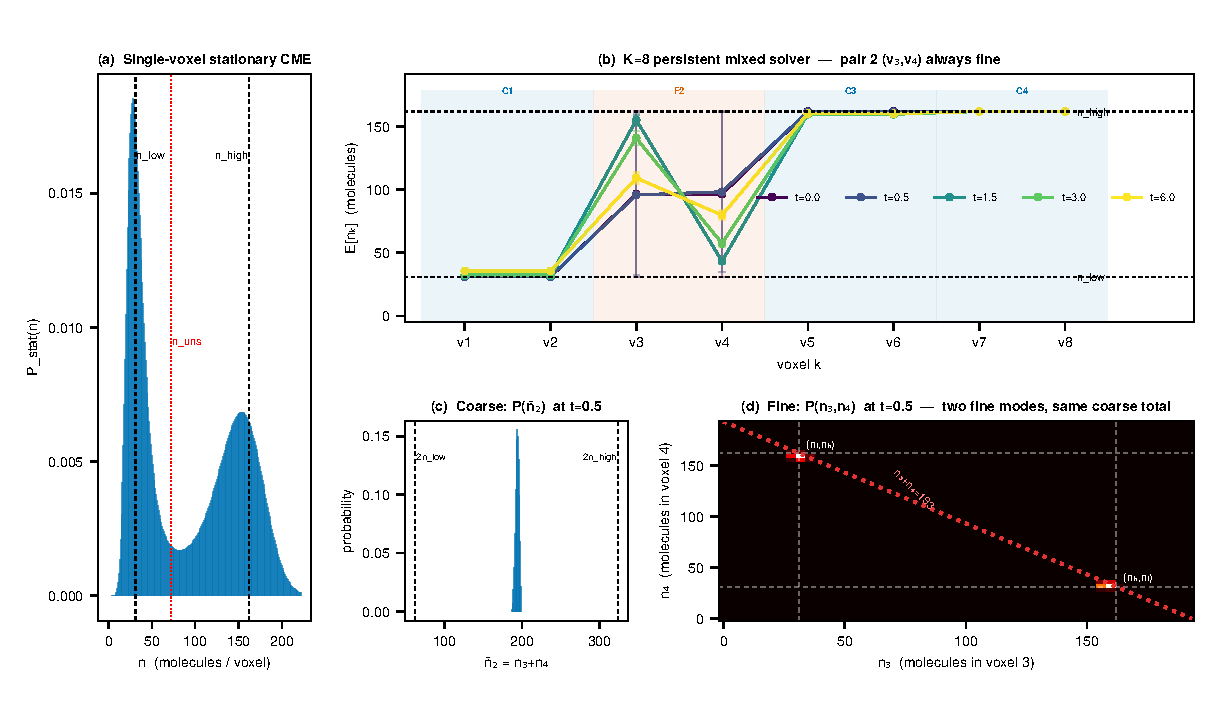
\includegraphics[width=\textwidth,height=0.65\textheight,keepaspectratio]{fig_k8_persistent}
  \end{center}

  {\footnotesize
  IC: interface neighbors~2 as equal superposition of $(n_l,n_h)$ and $(n_h,n_l)$.
  \textbf{(c)}~Coarse $P(\bar n_2)$: single peak at $193$ — orientation is lost.
  \textbf{(d)}~Fine $P(n_3,n_4)$: two modes along $n_3{+}n_4{=}193$ — the mixed state
  retains the within-pair structure.
  Full $K{=}8$ fine solve: intractable ($>258\mathrm{k}$ states).}

\end{frame}


\begin{frame}{Mixed generator is self-consistent}

  \textbf{Question:} does the fine/grouped coupling in $A^M$ introduce systematic error?

  \begin{center}
    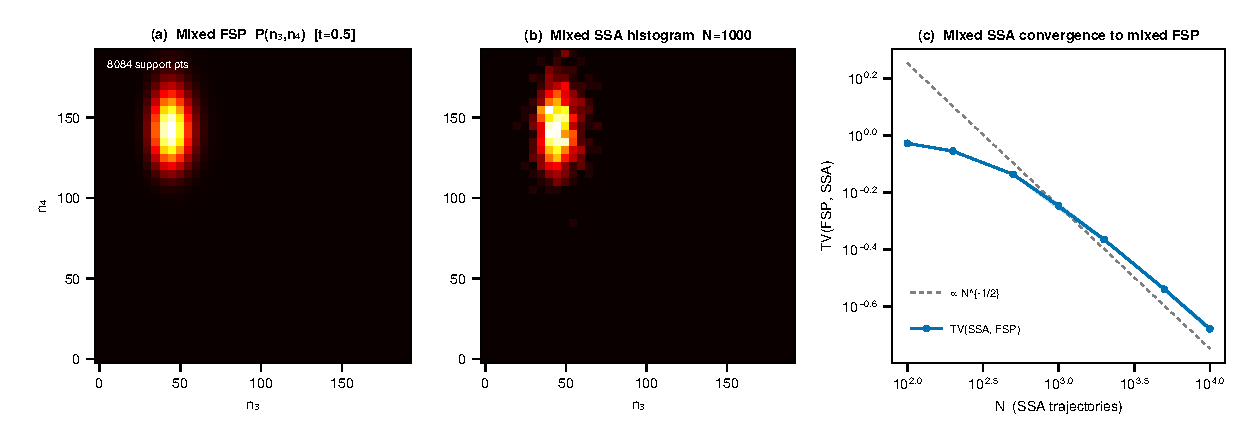
\includegraphics[width=\textwidth,height=0.56\textheight,keepaspectratio]{fig_mixed_fsp_ssa}
  \end{center}

  {\footnotesize
  Direct ODE solve on mixed state $(\bar n_1,n_3,n_4)$
  vs.\ Monte Carlo simulation on the same generator.
  Means agree to ${<}1\%$; TV $\sim N^{-1/2}$ (sampling noise only).}

\end{frame}


% ================================================================
\section{Summary}
% ================================================================


\begin{frame}[shrink=3]{Summary}

  \begin{block}{1. The RDME state space is exponential; diffusion enables grouping.}
    When diffusion between two neighboring voxels is fast relative to reactions,
    it equilibrates their joint distribution to $\Bin(\bar n, \frac{1}{2})$.
    Grouping = replacing $(n_1,n_2)$ by $\bar n = n_1{+}n_2$: exact marginalization $\calR$,
    Binomial split-back $\calP$.
    State space: $n_{\max}^K \to n_{\max}^{K/2}$.
  \end{block}

  \begin{block}{2. Grouping fails at a bistable front.}
    Reactions keep neighboring voxels in opposite stable states — faster than diffusion
    can equilibrate them. The imbalance criterion
    $\alpha_j = |\mu_{2j-1}-\mu_{2j}|/(\mu_{2j-1}+\mu_{2j})$
    detects this: large $\alpha_j$ means do not group pair $j$.
  \end{block}

  \begin{block}{3. Adaptive mixed-resolution evolution.}
    Keep a fine window around the front (exact within-pair distribution);
    group the rest (Binomial split-back valid where diffusion dominates).
    Evolve $\dot p^M = A^M p^M$ directly; reassign only when the front crosses a pair boundary.
  \end{block}

  \medskip
  \textbf{Open questions:} replace $\alpha_j$ with a rigorous diffusion flux-balance bound;
  multi-species; deeper hierarchies.

\end{frame}


% ================================================================
\appendix
\section{Appendix}
% ================================================================


\begin{frame}[shrink=22]{A naive approach: restrict-then-prolong at every step}

  \textbf{What if we grouped all pairs, solved the grouped ODE, then split back each step?}

  \begin{columns}[T]
    \begin{column}{0.52\textwidth}
      \begin{block}{Naive V-cycle over time step $\Delta t$}
        \begin{enumerate}\setlength\itemsep{0.5em}
          \item \textbf{Smooth} — apply within-group diffusion
            until the conditional equilibrates:
            \[ \tilde p = e^{\tau A_\mathrm{diff,\,within}}\,p. \]
          \item \textbf{Marginalize} — sum within pairs:
            \[ p^c = \calR\,\tilde p,\qquad
               \calR_{\bar n,\,s} = \mathbf{1}[n_1{+}n_2{=}\bar n]. \]
          \item \textbf{Grouped solve} — advance the grouped ODE:
            \[ \tilde p^c = e^{\Delta t\,\bar A}\,p^c. \]
          \item \textbf{Split back} — reconstruct within-pair split:
            \[ p_{\mathrm{new}} = \calP\,\tilde p^c,\qquad
               \calP_{s,\,\bar n} = \Bin\!\bigl(\bar n,\tfrac{1}{2}\bigr). \]
        \end{enumerate}
      \end{block}
    \end{column}
    \begin{column}{0.44\textwidth}
      \begin{center}
      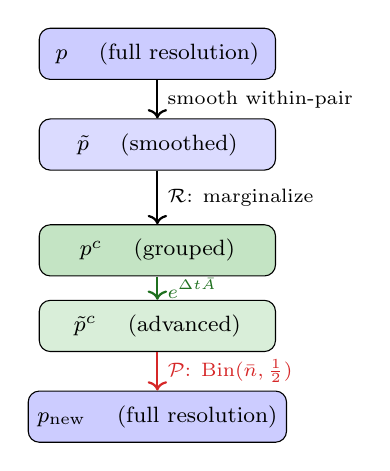
\begin{tikzpicture}[every node/.style={font=\footnotesize},scale=0.96]
        \node[draw,rounded corners,fill=blue!20,
              minimum width=3.0cm,minimum height=0.65cm]
          (f1) at (0,4.4) {$p$ \quad (full resolution)};
        \node[draw,rounded corners,fill=blue!14,
              minimum width=3.0cm,minimum height=0.65cm]
          (f2) at (0,3.2) {$\tilde p$ \quad (smoothed)};
        \node[draw,rounded corners,fill=coarsegreen!28,
              minimum width=3.0cm,minimum height=0.65cm]
          (c1) at (0,1.8) {$p^c$ \quad (grouped)};
        \node[draw,rounded corners,fill=coarsegreen!18,
              minimum width=3.0cm,minimum height=0.65cm]
          (c2) at (0,0.8) {$\tilde p^c$ \quad (advanced)};
        \node[draw,rounded corners,fill=blue!20,
              minimum width=3.0cm,minimum height=0.65cm]
          (f3) at (0,-0.4) {$p_\mathrm{new}$ \quad (full resolution)};
        \draw[->,thick] (f1.south) -- (f2.north)
          node[midway,right,font=\scriptsize]{smooth within-pair};
        \draw[->,thick] (f2.south) -- (c1.north)
          node[midway,right,font=\scriptsize]{$\calR$: marginalize};
        \draw[->,thick,coarsegreen!70!black] (c1.south) -- (c2.north)
          node[midway,right,font=\scriptsize]{$e^{\Delta t\bar A}$};
        \draw[->,thick,slowred] (c2.south) -- (f3.north)
          node[midway,right,font=\scriptsize]{$\calP$: Bin$(\bar n,\tfrac12)$};
      \end{tikzpicture}
      \end{center}
    \end{column}
  \end{columns}

  \begin{alertblock}{Step 4 fails at the front}
    Binomial split-back applies to \emph{all} pairs — including the front, where
    the conditional is not Binomial. \textbf{Solution:} evolve the mixed state $p^M$ directly
    (no split-back step at all).
  \end{alertblock}

\end{frame}


\begin{frame}[shrink=8]{Interface detection indicators}

  \begin{block}{Within-pair imbalance: front inside pair $j$}
    \[
      \alpha_j = \frac{|\mu_{2j-1} - \mu_{2j}|}{\mu_{2j-1}+\mu_{2j}}
    \]
    Large when the two voxels in pair $j$ are imbalanced — diffusion has not equilibrated them.
  \end{block}

  \begin{block}{Between-pair imbalance: front at a pair boundary}
    \[
      \beta_j  = \frac{|\mu_{2j} - \mu_{2j+1}|}{\mu_{2j}+\mu_{2j+1}}
    \]
    Large when voxels $2j$ and $2j{+}1$ (straddling a pair boundary) are imbalanced.
  \end{block}

  \begin{block}{Effective indicator and grouping rule}
    \[
      \alpha^\mathrm{eff}_j = \max(\alpha_j,\,\beta_{j-1},\,\beta_j).
    \]
    Flag group $j$ fine if $\alpha^\mathrm{eff}_j > \alpha_\mathrm{hi}$.
    Coarsen group $j$ only if $\alpha^\mathrm{eff}_j < \alpha_\mathrm{lo}$ (hysteresis).
  \end{block}

\end{frame}


\begin{frame}[shrink=6]{Representative configurations}

  \begin{center}
    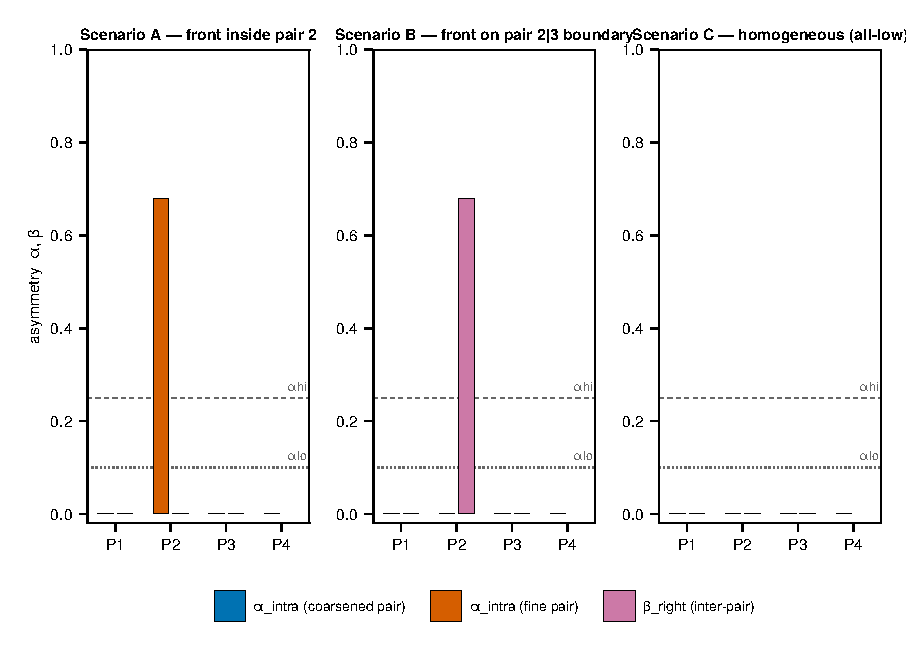
\includegraphics[width=\textwidth,height=0.78\textheight,keepaspectratio]{fig_adaptive_criterion}
  \end{center}
  {\footnotesize
  \textbf{A:} front interior to pair 2, detected by $\alpha_2$.\;
  \textbf{B:} front on the pair 2$|$3 boundary, detected by $\beta_2$.\;
  \textbf{C:} uniform — all pairs grouped.}

\end{frame}


\begin{frame}[allowframebreaks]{References}
  \footnotesize
  \begin{itemize}
    \item Erban, Chapman, Maini (2007). Stochastic simulations of reaction-diffusion.
      \textit{arXiv:0704.1908}.
    \item Munsky \& Khammash (2006). Finite State Projection.
      \textit{J.\ Chem.\ Phys.}, 124:044104.
    \item Kemeny \& Snell (1960). \textit{Finite Markov Chains}. Van Nostrand.
    \item Briggs, Henson, McCormick (2000). \textit{A Multigrid Tutorial}, 2nd ed.\ SIAM.
    \item Dendukuri, Chandrasekaran, Petzold (2025).
      Adaptive multigrid FSP for the RDME. \textit{In preparation}.
  \end{itemize}
\end{frame}

\end{document}
